\documentclass{beamer}

\mode<presentation>
{
  \usetheme{CambridgeUS}
  % \setbeamercovered{transparent}
}

\usepackage[T1]{fontenc}
\usepackage[utf8]{inputenc}
\usepackage[spanish]{babel}
\usepackage{color}
\usepackage{hyperref}
\usepackage{algorithm,algorithmic}
\usepackage{colortbl}
\usepackage{graphicx}
\usepackage{multicol}
\usepackage{enumitem}
\setitemize{itemsep=1.2em,%
  label=\usebeamerfont*{itemize item}%
  \usebeamercolor[fg]{itemize item}%
  \usebeamertemplate{itemize item}
}

\usepackage{minted}
\usepackage[skins,minted]{tcolorbox}

\newcommand{\code}[1]{\mintinline{java}{#1}}
\newcommand{\codet}[1]{\texttt{#1}}

\setminted[java]{
  linenos=true,
  fontfamily=tt,
  fontsize=\small,
  frame=leftline,
  autogobble=True,
}

\newminted[jsmall]{java}{
  fontsize=\footnotesize
  , linenos = false
  , frame=single
  , autogobble=true
}

\newtcblisting{java}[2][]{
  minted language=java,
  enhanced, listing engine=minted,
  listing only, #1, title=#2, left=2em
}

\setminted[bash]{
  linenos=true,
  fontfamily=tt,
  fontsize=\small,
  frame=leftline
}

\newtcblisting{bash}[2][]{minted language=bash,
  enhanced, listing engine=minted,
  listing only, #1, title=#2, left=2em
}

\title[\textbf{Programación 2}]{\textbf{Programación 2}}
\subtitle{Herencia y Clases Abstractas}

\author[IF-EG]
{Profesores:\\
  Ismael Figueroa -  \texttt{\small ifigueroap@gmail.com} \\
  \vspace{0.5mm} \\
  Eduardo Godoy - \texttt{\small eduardo.gl@gmail.com}
}

\institute[Universidad de Valparaíso]

\date{}

\begin{document}

\begin{frame}
  \titlepage
\end{frame}

\section{Herencia}

\begin{frame}
  \frametitle{¿Qué es la herencia?}
  \begin{itemize}
  \item Es un mecanismo para \emph{definir nuevas clases en base a
      otras ya existentes}
    
  \item A la clase existente se le llama: clase base, superclase, o
    clase padre. A la clase nueva se le llama: clase extendida,
    subclase, o clase hija
    
  \item La subclase \emph{hereda} o \emph{adquiere} todos los
    atributos y métodos de la superclase
    
  \item La subclase puede usar el constructor de la super clase
    mediante la palabra clave \codet{super}
    
  \end{itemize}
\end{frame}

\begin{frame}[fragile]
  \frametitle{Ejemplo de Herencia}

     \begin{columns}
       \begin{column}{0.45\textwidth}
         \begin{jsmall}
           public class Rectangulo {
             Integer largo, ancho;

             public Rectangulo(Integer l,
                               Integer a) {
              largo = l;
              ancho = a;                               
             }

             public Integer area() {
               return largo*ancho;
             }

             public Integer perimetro() {
               return 2*(ancho + largo);
             }
           }           
         \end{jsmall}
     \end{column}
    % 
    \begin{column}{0.55\textwidth}      
      \begin{jsmall}
        public class Cuadrado
        extends Rectangulo {
          /* Hereda: largo, ancho,
          area y perimetro */
          public Cuadrado(Integer lado) {
            super(lado, lado);
          }
        }

        public class Main {
          public static
          void main(String[] args) {
            Rectangulo r = new Rectangulo(4,2);
            Cuadrado c   = new Cuadrado(5);
            /* ... */
          }
        }
      \end{jsmall}      
    \end{column}
  \end{columns}  
  
\end{frame}

\begin{frame}
  \frametitle{Especialización de la subclase}

  \begin{itemize}
  \item Se dice que la superclase \emph{es más general} que la
    subclase
    
  \item Al reves, la subclase \emph{es una especialización} de la
    superclase
    
  \item La herencia se usa para codificar relaciones \emph{``es
      un''}. Por ejemplo: \emph{un Cuadrado \textbf{es un} Rectángulo}
    
  \item Al ser más específica, una subclase puede agregar nueva
    información mediante \emph{nuevos atributos} y \emph{nuevos
      métodos}
    
  \item Una subclase también puede ser más específica al
    \textbf{\textit{sobre-escribir}} métodos de la superclase. Se usa
    la anotación \codet{@Override} para que el compilador sepa nuestra
    intención!
    
  \end{itemize}
\end{frame}

\begin{frame}[fragile]
  \frametitle{Especialización: nuevos atributos}

     \begin{columns}
       \begin{column}{0.45\textwidth}
         \begin{jsmall}
           public class Rectangulo {
             Integer largo, ancho;

             public Rectangulo(Integer l,
                               Integer a) {
              largo = l;
              ancho = a;                               
             }

             public Integer area() {
               return largo*ancho;
             }

             public Integer perimetro() {
               return 2*(ancho + largo);
             }
           }           
         \end{jsmall}
     \end{column}
    % 
    \begin{column}{0.55\textwidth}      
      \begin{jsmall}
        public class RectColor
        extends Rectangulo {
          String color;

          public RectColor(Integer l,
                           Integer a,
                           String color) {
              super(l, a);
              this.color = color;                                   
          }
        }

        public class Main {
          public static
          void main(String[] args) {
            RectColor rc;
            rc = new RectColor("Rojo", 4, 2);
            /* ... */
          }
        }
      \end{jsmall}      
    \end{column}
  \end{columns}  
\end{frame}

\begin{frame}[fragile]
  \frametitle{Especialización: nuevos métodos}

     \begin{columns}
       \begin{column}{0.45\textwidth}
         \begin{jsmall}
           public class Rectangulo {
             Integer largo, ancho;

             public Rectangulo(Integer l,
                               Integer a) {
              largo = l;
              ancho = a;                               
             }

             public Integer area() {
               return largo*ancho;
             }

             public Integer perimetro() {
               return 2*(ancho + largo);
             }
           }           
         \end{jsmall}
     \end{column}
    % 
    \begin{column}{0.55\textwidth}      
      \begin{jsmall}
        public class RectColor
        extends Rectangulo {
          String color;
          /* ... constructor ...*/

          public void setColor(String c) {
            color = c;
          }
        }

        public class Main {
          public static
          void main(String[] args) {
            RectColor rc;
            rc = new RectColor("Rojo", 4, 2);
            rc.setColor("Verde");
            /* ... */
          }
        }
      \end{jsmall}      
    \end{column}
  \end{columns}  
\end{frame}

\begin{frame}[fragile]
  \frametitle{Especialización: \textbf{sobreescribir} métodos}

  Cuando una subclase sobreescribe un método de una superclase estamos
  asociando un comportamiento más específico a una misma acción que en
  la superclase es más general. Lo clásico que hemos visto hasta ahora
  es sobreescribir el método \codet{toString()}, que viene
  transitivamente desde la superclase \codet{Object}.

  \begin{jsmall}
    public class Rectangulo {
      Integer largo, ancho;
      /* ... */

      @Override // no olvidar el override!
      public String toString() {
        return String.format(
           "Un hermoso rectangulo de largo %d y %ancho %d", largo, ancho);
      }
    }    
  \end{jsmall}  
\end{frame}

\begin{frame}[fragile]
  \frametitle{Ejemplo: Figuras Geométricas}

  Podemos ir más allá de los rectángulos a una jerarquía de clases más
  completa, considerando una clase \codet{Figura}, especializada en
  \codet{Figura2D}, y \codet{Figura3D}, y figuras concretas en cada
  caso....

  \begin{center}
  \begin{figure}
    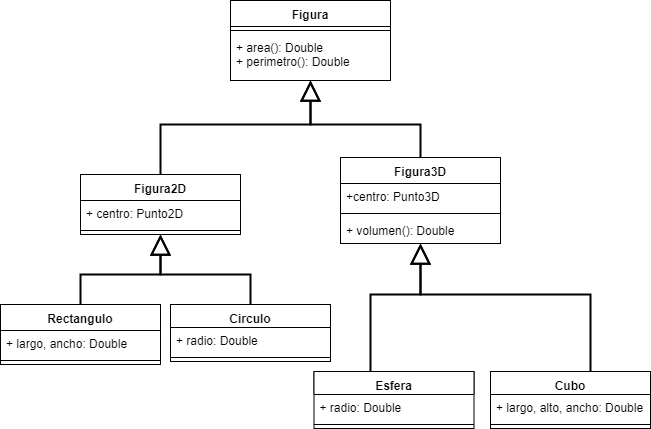
\includegraphics[scale=0.4]{figures/Figuras.png}
  \end{figure}
  \end{center}

\end{frame}

\begin{frame}[fragile]
  \frametitle{Métodos destinados a ser sobreescritos}

  Para la clase \codet{Figura}, es imposible saber cuál es una buena
  implementación para \codet{area} y \codet{perimetro}, ya que
  dependen de información específica de cada figura...

  \begin{jsmall}
    public class Figura {
      public Double area() {
        /* ??? */
      }

      public Double perimetro() {
        /* ??? */
      }
    }
  \end{jsmall}
\end{frame}

\begin{frame}[fragile]
  \frametitle{Métodos destinados a ser sobreescritos}

  Una opción es arrojar una excepción:

  \begin{jsmall}
    public class Figura {
      public Double area() {
       throw new UnsupportedOperationException("Debe refinar en subclases");
     }

     /* ... */
    }
  \end{jsmall}

  Pero esto es ``trampa'', porque en realidad queremos decir que todas
  las figuras deben implementar, según su contexto, los métodos
  \codet{area} y \codet{perimetro}
\end{frame}

\section{Métodos y Clases Abstractos}

\begin{frame}
  \frametitle{Métodos Abstractos}

  \begin{itemize}
  \item Son métodos en los que solo se declara su tipo de retorno,
    nombre, y parámetros, \textbf{\textit{pero que no tienen
        implementación}}.
    
  \item Se definen cuando se requiere que una subclase complete ese
    método con una implementación concreta y específica
    
  \item Si una clase incluye un método abstracto, entonces
    obligatoriamente \textbf{\textit{la clase también debe ser
        abstracta}}
    
  \end{itemize}
  
\end{frame}

\begin{frame}
  \frametitle{Clases Abstractas}

  \begin{itemize}
  \item Son clases diseñadas para \emph{nunca ser instanciadas}!!
    
  \item Su propósito es funcionar como superclase en una jerarquía de
    herencia
    
  \item Una clase abstracta puede declarar ``piezas faltantes'' que
    \textbf{deben} ser implementadas por las subclases para
    convertirse en una \emph{clase concreta}
    
  \item Las piezas faltantes pueden ser atributos y principalmente
    métodos abstractos    
  \end{itemize}
\end{frame}

\begin{frame}[fragile]
  \frametitle{Una \codet{Figura} abstracta}

  \begin{jsmall}
    public abstract class Figura {
      public abstract Double area();
      public abstract Double perimetro();
    }

    public class Punto2D {
      Integer x, y;
      public Punto2D(Integer x, Integer y) {
        this.x = x;
        this.y = y;
      }      
    }

    public class Figura2D extends Figura {
      public Punto2D centro;
      public Figura2D(Punto2D centro) {
        this.centro = centro;
      }
    }
  \end{jsmall}
\end{frame}

\begin{frame}[fragile]
  \frametitle{Un \codet{Rectangulo} concreto}
  \begin{jsmall}
    public class Rectangulo extends Figura2D {
      Integer largo, ancho;
      public Rectangulo(Punto2D centro, Integer largo, Integer ancho) {
        this.centro;
        this.largo = largo;
        this.ancho = ancho;
      }

      @Override
      public Double area() {
        return largo * ancho;
      }

      @Override
      public Double perimetro() {
        return 2*(largo + ancho);
      }        
    }
  \end{jsmall}  
\end{frame}

\section{Control de Acceso con Herencia}

\begin{frame}[fragile]
  \frametitle{Variables \codet{public}}

Observe el código de \codet{Figura2D}:

\begin{jsmall}
public class Figura2D extends Figura {
  public Punto2D centro;
  public Figura2D(Punto2D centro) {
    this.centro = centro;
  }
}
\end{jsmall}

El atributo es \codet{public} por lo que cualquier usuario de nuestra
librería de figuras podría cambiar la posición de una figura. Esto
ciertamente no es deseable, pero ...

\end{frame}

\begin{frame}[fragile]
  \frametitle{Variables \codet{private}}

Si hacemos que el centro sea \codet{private}, tendremos un error en:

\begin{jsmall}
public Rectangulo(Punto2D centro, Integer largo, Integer ancho) {
  this.centro;
  this.largo = largo;
  this.ancho = ancho;
}
\end{jsmall}

El error nos dice que \textbf{\textit{no podemos acceder al atributo
    \codet{centro}}}!! Pero se suponía que por herencia obteníamos
todo...

En Java las variables \codet{private} están ocultas en las subclases,
y sólo se pueden acceder mediante los métodos de la superclase que los
manipulan...

\end{frame}

\begin{frame}
  \frametitle{Nuevo acceso: variables \codet{protected}}

  Java incorpora un nuevo modificador de acceso: \codet{protected}

  \begin{itemize}
  \item Permite que el campo sea visible en las subclases
    
  \item Mantiene el nivel de acceso dentro de la misma clase y el
    mismo paquete
    
  \item Para el resto del mundo, es como un atributo privado

  \item Ver \url{docs.oracle.com/javase/tutorial/java/javaOO/accesscontrol.html}
    
  \end{itemize}
  
\end{frame}

\section{Ejercicio}

\begin{frame}[fragile]
  \frametitle{Codificación Figuras Geométricas}

  \begin{small}
    Codifique el modelo de clases que representa las figuras
    geométricas. Escriba un programa principal que construya una
    instancia de cada clase concreta, y donde se invoquen todos sus
    métodos. Use clases y métodos abstractos según corresponda. Todos
    los atributos de clase deben tener acceso \codet{protected}.
  \end{small}

  \begin{center}
  \begin{figure}
    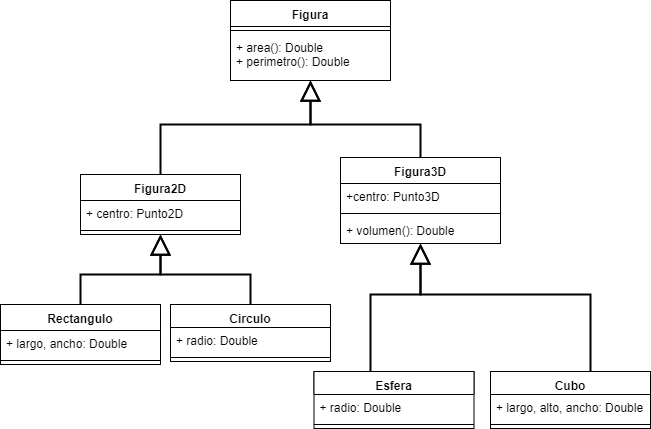
\includegraphics[scale=0.35]{figures/Figuras.png}
  \end{figure}
  \end{center}

\end{frame}

\begin{frame}
  \frametitle{Preguntas}
  \hspace{4cm}\huge{Preguntas?}  
\end{frame}

\end{document}